\begin{figure}
    \centering
    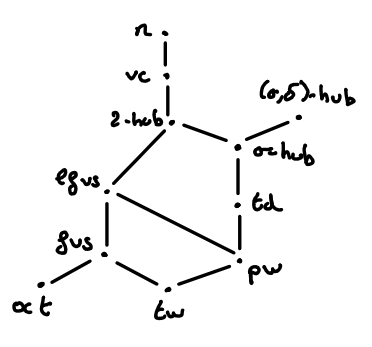
\includegraphics[width=.4\textwidth]{figures/hierarchy.png}
    \caption{Hierarchy of parameters. Parameters are arranged vertically from bottom to top based on their comparative scaling. Treewidth is positioned at the bottom, indicating one of the smallest parameter, while $n$ represents the number of vertices in the graph at the top. A line between two parameters signifies comparability.}
    \label{fig:hierarchy}
\end{figure}